\documentclass{beamer}

\usepackage{hyperref}

\usetheme{Antibes}

\title{Maintainable Embedded Linux Solutions}
\author{Thomas Irgang \and Simone Weiß}
\institute{EASTERHEGG 2024 - RABBIT PROTOTYPING}
\date{March 31, 2024}
\titlegraphic{
    
\includegraphics[width=2cm]{assets/logo.png}
}

\newcommand\pro{\item[$+$]}
\newcommand\con{\item[$-$]}

\begin{document}

\begin{frame}
    \titlepage
\end{frame}

\begin{frame}
	\begin{block}{Topic}
		How to build long-term secure and maintainable embedded Linux solutions
		while spending limited effort to keep the solution secure?
	\end{block}
\end{frame}

\section{Is Linux the right choice?}

\begin{frame}{Do I need Linux for my project?}
	\begin{block}{Rule}
		Smaller is better!
	\end{block}

	\begin{itemize}
		\item Less interfaces means less attack surface!
		\item Less software means less maintenance effort!
	\end{itemize}

	\begin{tabular}{cccc}
	&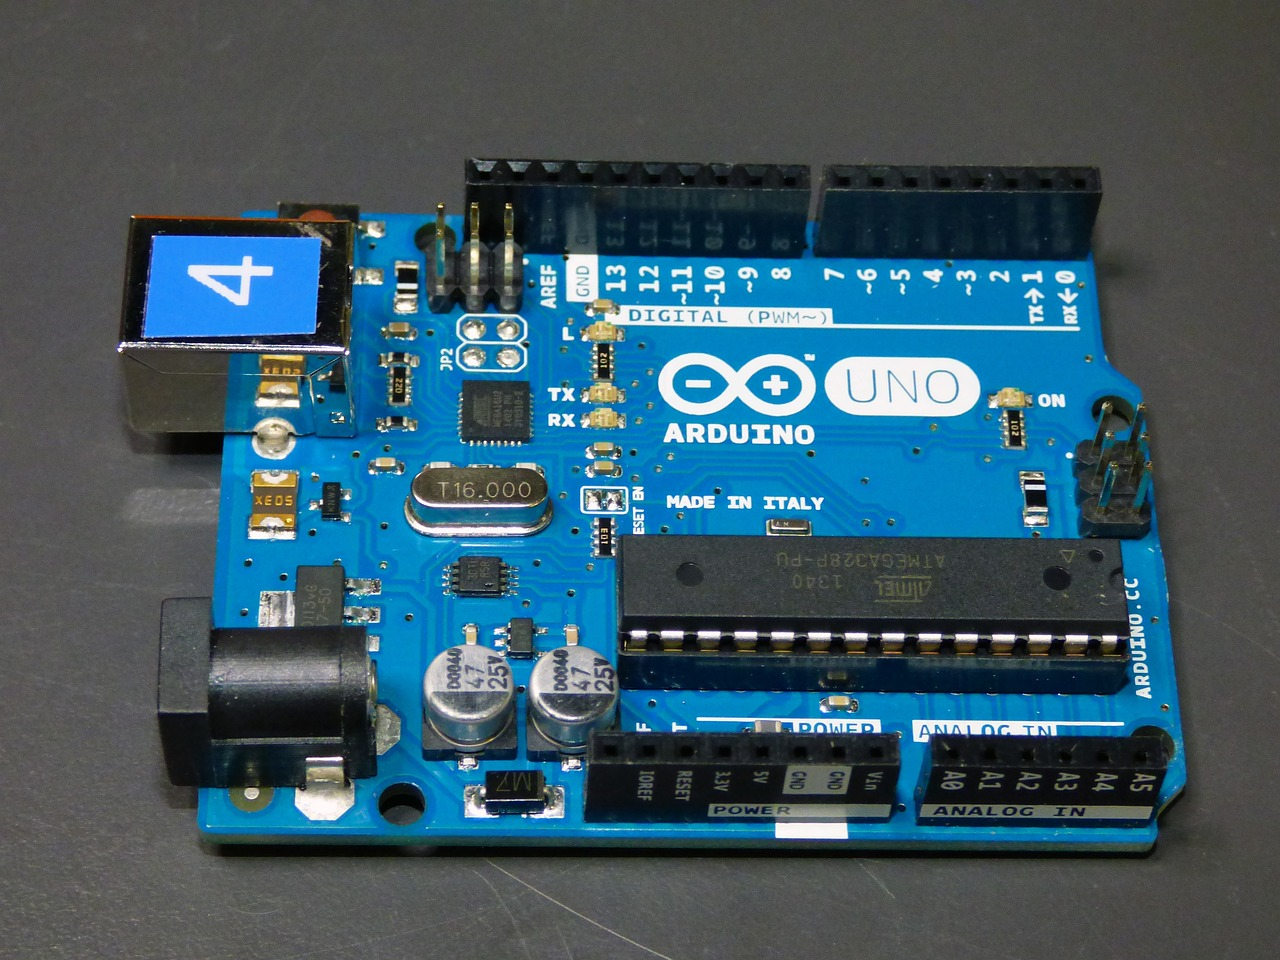
\includegraphics[width=1.9cm]{assets/Pixabay_Arduino_integrated-circuit-441289_1280.jpg} &
	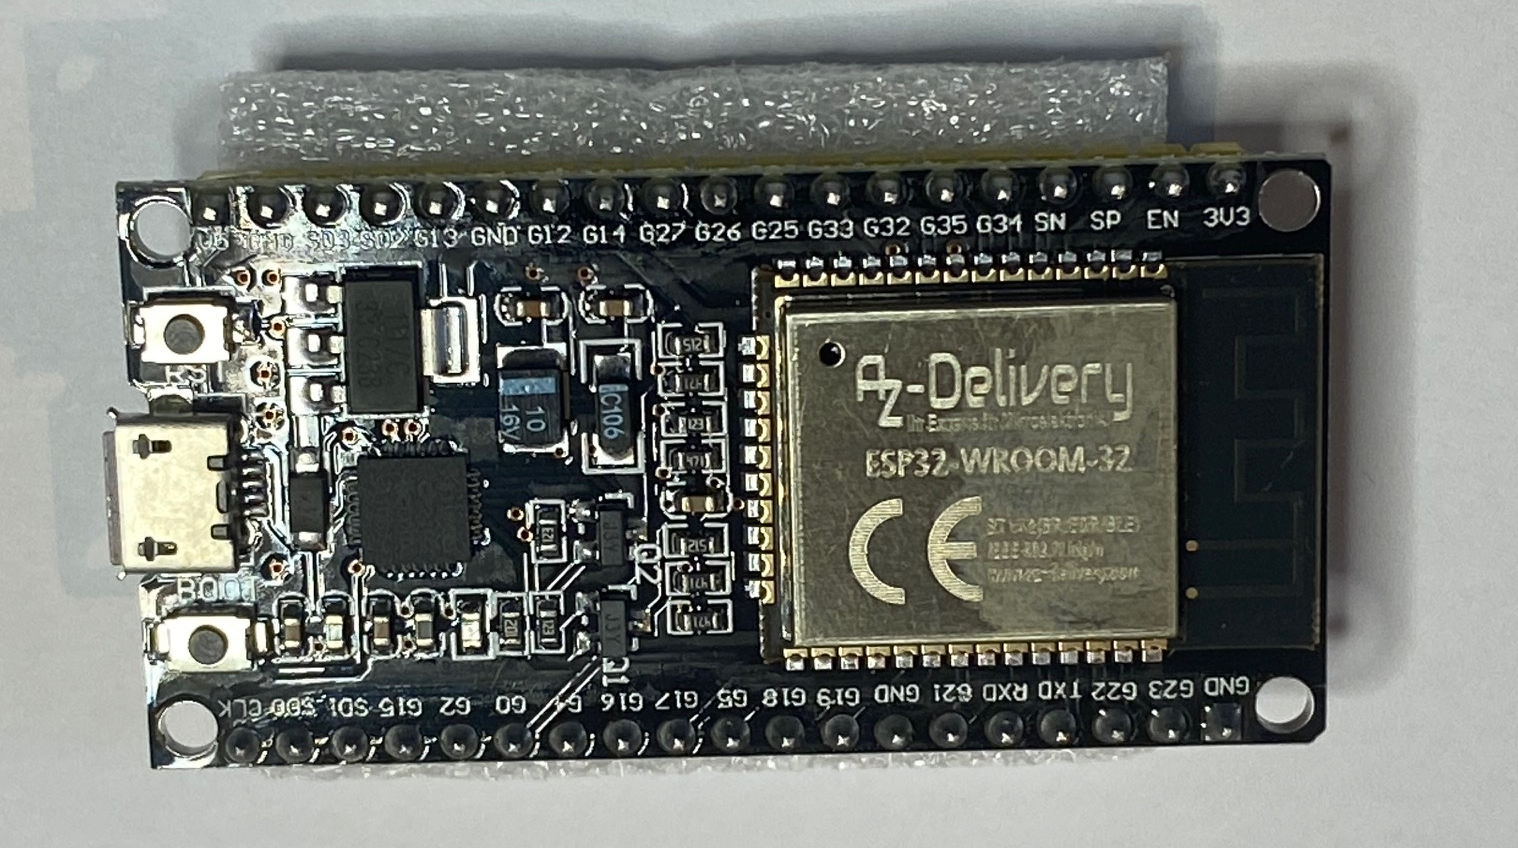
\includegraphics[width=1.9cm]{assets/ESP32.png} & 
	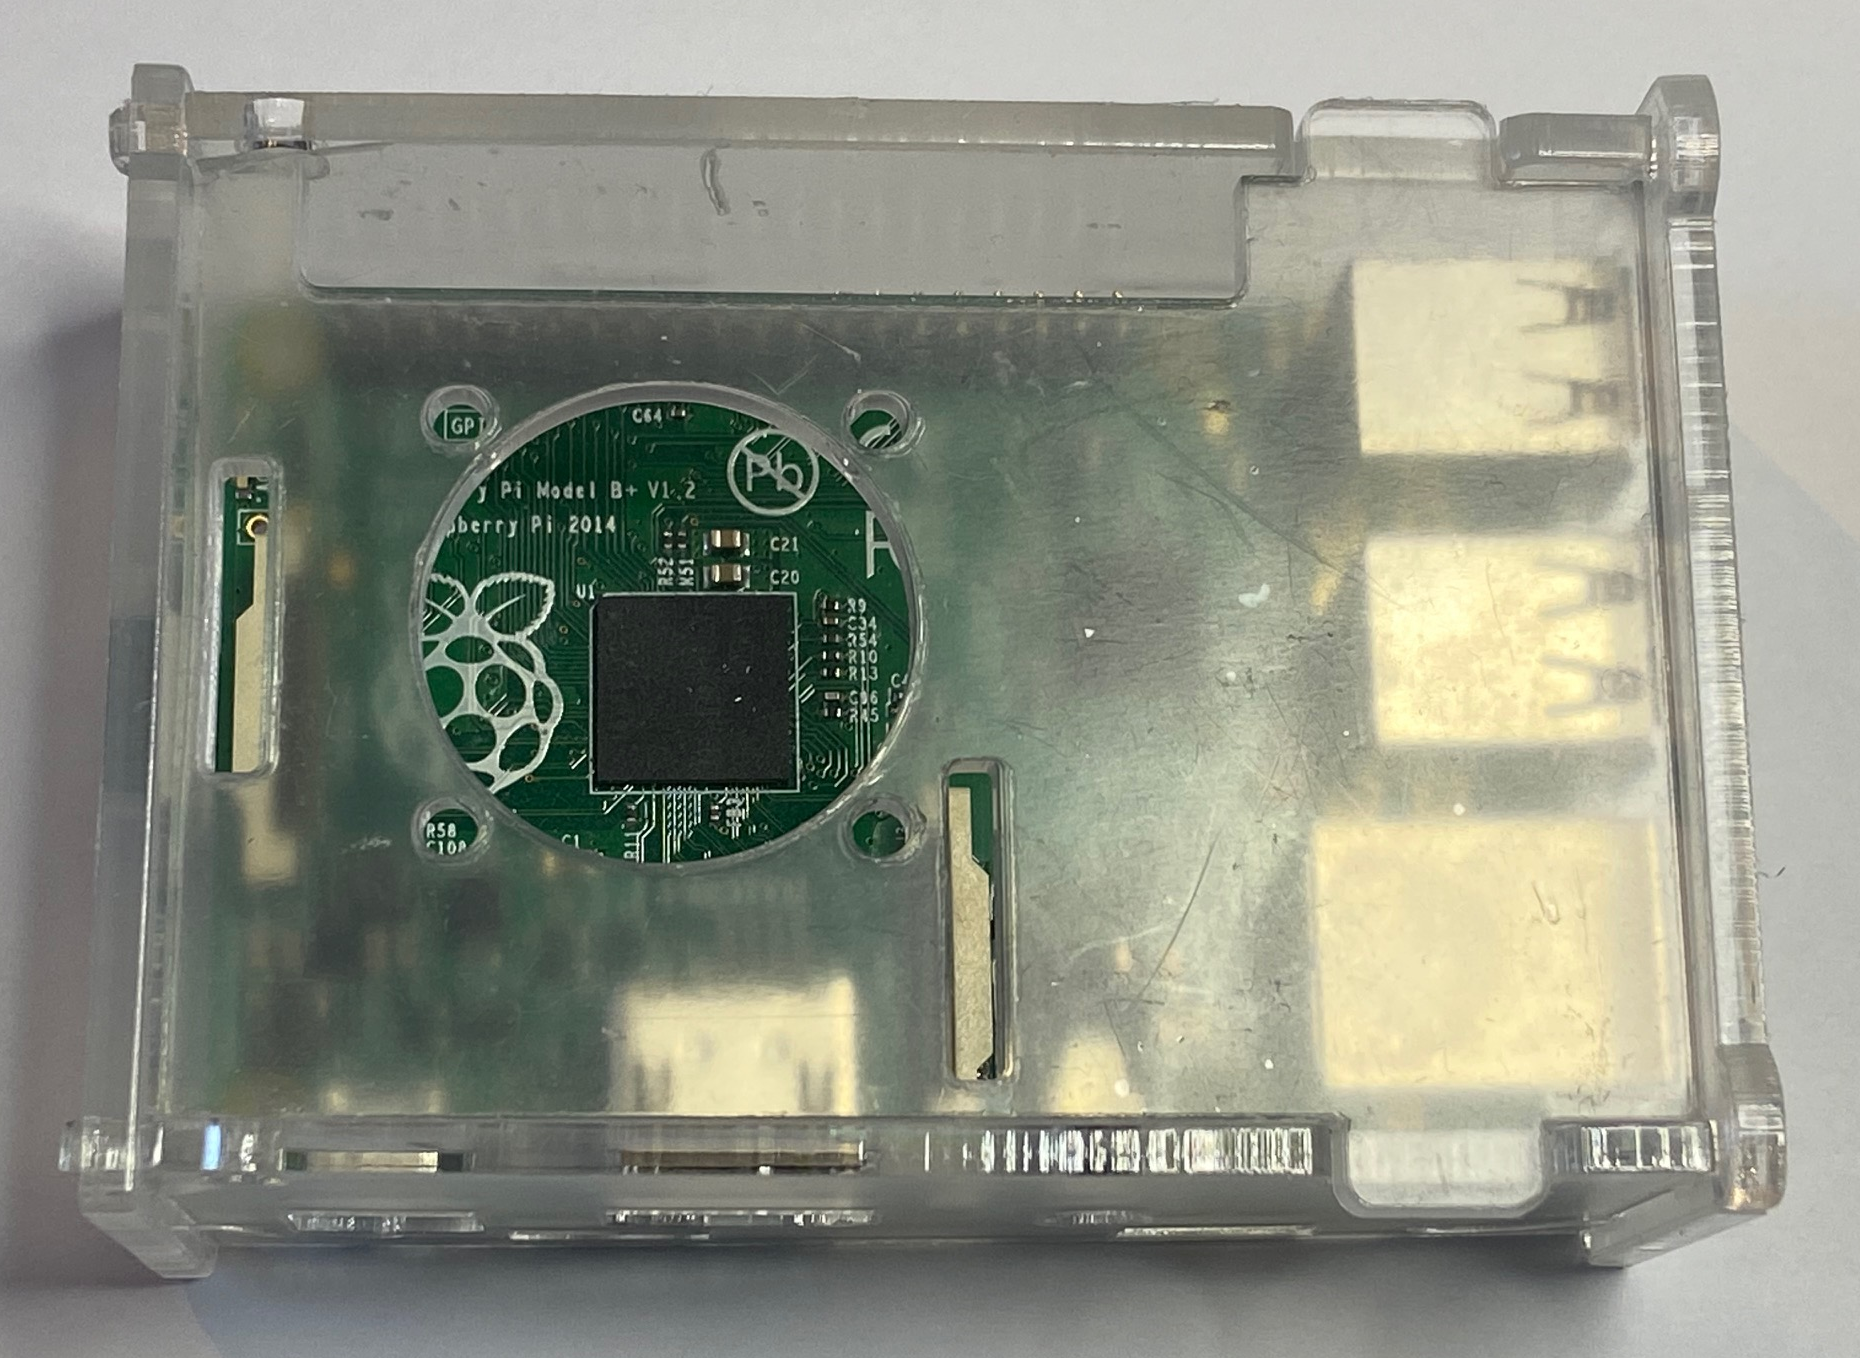
\includegraphics[width=1.9cm]{assets/Raspberry_Pi.png} \\
	&\textbf{Arduino} & \textbf{ESP32 FreeRTOS} & \textbf{SBC Linux} \\
	real-time & + &  + & - \\
	energy & + & o & - \\
	communication & - & o & + \\
	\end{tabular}
\end{frame}

\begin{frame}{What's the life-time of my project?}
	\begin{block}{What's the life-time?}
		Do you need to care about maintenance and updates?
	\end{block}

	\begin{columns}
    \column{0.33\textwidth}
        \centering
        \textbf{Experiment}
        \begin{itemize}
        		\item few months
        		\item no maintenance
        		\item some reusability
        \end{itemize}
    \column{0.33\textwidth}
        \centering
        \textbf{Media-Center}
        \begin{itemize}
        		\item some years
        		\item typical IT distribution maintenance
        		\item no reusability needed
        \end{itemize}
    \column{0.34\textwidth}
        \centering
        \textbf{Home Automation}
        \begin{itemize}
        		\item more than 15 years
        		\item maintenance and upgrades
        		\item reusability for mid-term upgrade needed
        \end{itemize}
    \end{columns}
\end{frame}

\section{Embedded Linux}

\begin{frame}{How to build an embedded Linux?}
	\begin{block}{Topic}
		How to build a project specific solution using embedded Linux?
	\end{block}

	\begin{itemize}
		\item "golden image"
		\item "from scratch"
		\item "as a remix"
	\end{itemize}
\end{frame}

\begin{frame}{The "golden image" approach}
	\begin{itemize}
		\item starting from an existing Linux image, e.g. Raspberry Pi OS,
		\item install the required tools,
		\item and configure it,
		\item and freeze the image.
	\end{itemize}

	\begin{columns}
    \column{0.5\textwidth}
        \centering
        \begin{itemize}
			\pro easy approach
			\pro maintained by used distribution
		\end{itemize}        
    \column{0.5\textwidth}
        \centering
        \begin{itemize}
        		\con solution and base distribution are mixed
        		\con no support for variants
        		\con lots of not needed software
        \end{itemize}
    \end{columns}
\end{frame}

\begin{frame}{The "from scratch" approach}
	\begin{itemize}
		\item using a built toolkit, e.g. Yocto or Buildroot
		\item which builds all packages from source
		\item using a project specific configuration and patches
	\end{itemize}

	\begin{columns}
    \column{0.5\textwidth}
        \centering
        \begin{itemize}
        	\pro optimal system
        	\pro minimized resources
        	\pro reusable solution
        	\pro support for variants
        \end{itemize}
    \column{0.5\textwidth}
        \centering
        \begin{itemize}
        		\con learning curve
        		\con maintenance effort
        \end{itemize}
    \end{columns}
\end{frame}

\begin{frame}{The "remix" approach}
	\begin{itemize}
		\item use the packages from an existing distribution
		\item and create a solution-specific remix
		\item by reusing the exiting binary packages
		\item to build a custom image with customized configuration
	\end{itemize}

	\begin{columns}
		\column{0.5\textwidth}
		\centering
		\begin{itemize}
			\pro low maintenance effort
			\pro smaller than "golden image"
			\pro reusable solution
			\pro support for variants
		\end{itemize}
		\column{0.5\textwidth}
		\centering
		\begin{itemize}
			\con learning curve
			\con limited optimization
		\end{itemize}
	\end{columns}
\end{frame}

\section{The source build toolkit}

\begin{frame}
	\begin{block}{Topic}
		How can I efficient build a customized embedded Linux distribution from scratch?
	\end{block}
\end{frame}

\begin{frame}{Tools for source builds}
	\begin{tabular}{c|ccc}
		& \textbf{Yocto} & \textbf{Buildroot}  \\
		\hline
		% TODO: compare Yocto and Buildroot
	\end{tabular}
\end{frame}

\begin{frame}{Yocto}
	\begin{block}{Whats included?}
		Provides Metadata (recipes, configuration, data how things are built), BitBake (buildsystem) to build a custom embedded Linux distribution and a SDK. It also provides Poky as a reference distribution. Layer for many boards available
	\end{block}

	\begin{itemize}
		\item Will build packages and images based on recipes and configuration
		\item Metadata is using Bash and Python
		\item Docs: \url{https://docs.yoctoproject.org/}
		\item Source: \url{git://git.yoctoproject.org/poky}
	\end{itemize}
\end{frame}

\begin{frame}{Yocto: Raspberry Pi image}
	\begin{itemize}
		\item Source: \href{https://git.yoctoproject.org/poky}{poky}, \href{https://git.yoctoproject.org/meta-raspberrypi/}{bsp}
		\item based on Poky
		\item Steps:
		\begin{itemize}
			\item install kas: pip3 install kas
			\item get kas.yml
			\item run kas build
			\item copy image to SD card
		\end{itemize}
		\item more details on \href{https://github.com/tomirgang/eh21_maintainable_linux/tree/main/examples/first_build_rpi4/yocto}{Github}
	\end{itemize}
\end{frame}

\begin{frame}{Buildroot}
	\begin{block}{Whats included?}
		Generate embedded Linux systems (Rootfs, Kernel, Bootloader, SDK)  based on a "Makefile collection" and configuration for a number of boards. Simpler then Yocto(easier, but less features)
	\end{block}

	\begin{itemize}
		\item Will build components and images from source
		\item Style is based on Makefile and Kconfig 
		\item Docs: \url{https://buildroot.org/downloads/manual/manual.html}
		\item Source: \url{https://gitlab.com/buildroot.org/buildroot/}
	\end{itemize}
\end{frame}

\begin{frame}{Buildroot: Raspberry Pi image}
	\begin{itemize}
		\item Source: \href{https://gitlab.com/buildroot.org/buildroot/}{GitLab}
		\item Steps:
		\begin{itemize}
			\item install \href{https://buildroot.org/downloads/manual/manual.html\#requirement}{dependencies}
			\item make raspberrypi4\_64\_defconfig
			\item make
			\item copy image to SD card
		\end{itemize}
		\item more details on \href{https://github.com/tomirgang/eh21_maintainable_linux/tree/main/examples/first_build_rpi4/buildroot}{Github}
	\end{itemize}
\end{frame}

\section{Remixing a distribution}

\begin{frame}
	\begin{block}{Topic}
		How can I efficient build a remix embedded Linux distribution?
	\end{block}
\end{frame}

\begin{frame}{Tools for building a remix distribution}
	\begin{tabular}{c|ccc}
		& \textbf{Elbe} & \textbf{Debos} & \textbf{Kiwi-ng} \\
		\hline
		target & Embedded Image & Debian remix & Linux remix \\ 
		format & deb & deb & deb, rpm, arch \\
		build packages & yes & no & no \\
	\end{tabular}
\end{frame}

\subsection{Kiwi-ng}

\begin{frame}{Kiwi-ng}
	\begin{block}{What's included?} 
		Kiwi-ng is a utility to build Linux system appliances. 
		An appliance is a ready to use image of an operating system including a pre-configured application for a specific use case. 
	\end{block}

	\begin{itemize}
		\item Supports all major package managers
		\item Image description using XML and config scripts
		\item Docs: \url{https://osinside.github.io/kiwi/}
		\item Source: \url{https://github.com/OSInside/kiwi}
	\end{itemize}
\end{frame}

\begin{frame}{Kiwi-ng: Raspberry Pi image}
	\begin{itemize}
		\item Source: \href{https://github.com/OSInside/kiwi-descriptions/tree/main/ubuntu/aarch64/ubuntu-jammy-rpi}{Github}
		\item based on Ubuntu Jammy
		\item Steps:
		\begin{itemize}
			\item install \url{https://pypi.org/project/kiwi/}
			\item install \url{https://pypi.org/project/kiwi-boxed-plugin/}
			\item get image description
			\item run image build
			\item copy image to SD card
		\end{itemize}
		\item more details on \href{https://github.com/tomirgang/eh21_maintainable_linux/tree/main/examples/first_build_rpi4/kiwi-ng}{Github}
	\end{itemize}
\end{frame}

\subsection{Debos}

\begin{frame}{Debos}
	\begin{block}{What's included?} 
		debos is a tool to make the creation of various Debian-based OS images simpler. While most other tools focus on specific use-cases, debos is more meant as a tool-chain to make common actions trivial while providing enough rope to do whatever tweaking that might be required behind the scene.
	\end{block}
	
	\begin{itemize}
		\item Supports only Debian packages
		\item Image description using YAML
		\item Docs: \url{https://pkg.go.dev/github.com/go-debos/debos}
		\item Source: \url{https://github.com/go-debos/debos}
	\end{itemize}
\end{frame}

\begin{frame}{Debos: Raspberry Pi image}
	\begin{itemize}
		\item Source: \href{https://github.com/go-debos/debos-recipes/tree/main/rpi64}{Github}
		\item based on Debian Bullseye
		\item Steps:
		\begin{itemize}
			\item Debian: install debos packages
			\item run image build
			\item copy image to SD card
		\end{itemize}
		\item more details on \href{https://github.com/tomirgang/eh21_maintainable_linux/tree/main/examples/first_build_rpi4/debos}{Github}
	\end{itemize}
\end{frame}

\subsection{Elbe}

\begin{frame}{Elbe}
	\begin{block}{What's included?} 
		Elbe is a Debian-based system to generate root filesystems for embedded devices.
	\end{block}

	\begin{itemize}
		\item Supports only Debian packages
		\item Image description using XML
		\item Docs: \url{https://elbe-rfs.org/docs/sphinx}
		\item Source: \url{https://github.com/Linutronix/elbe}
	\end{itemize}
\end{frame}

\begin{frame}{Elbe: Raspberry Pi image}
	\begin{itemize}
		\item Based on \href{https://github.com/Linutronix/elbe/blob/master/examples/arm64-qemu-virt.xml}{example arm64-qemu-virt}
		\item Steps:
		\begin{itemize}
			\item Debian: install elbe package
			\item prepare the initvm
			\item run the image build
			\item copy image to SD card
		\end{itemize}
		\item more details on \href{https://github.com/tomirgang/eh21_maintainable_linux/tree/main/examples/first_build_rpi4/elbe}{Github}
	\end{itemize}
\end{frame}

\section{Minimal image}

\begin{frame}{Which tool to use?}
	\begin{block}{Topic}
		What is the right tool?
	\end{block}

	\begin{itemize}
		\item Minimal image to compare the tools:
		\begin{itemize}
			\item QEMU
			\item Systemd 
			\item OpenSSH server
		\end{itemize}
	\end{itemize}
\end{frame}

\begin{frame}{Comparison of different tools}
	\begin{tabular}{c|ccccc}
		& \textbf{Build} & \textbf{Startup} & \textbf{Size} & \textbf{Processes} & \textbf{Packages} \\
		\hline
		Yocto & X s & X s & X MB & X & X \\ 
		Buildroot & X s & X s & X MB & X & X \\
		\hline
		Debos & 6:30 & ~14s & 701 MB & 64 & 143 \\
		Elbe & 7:19 & ~14s & 872 MB & 64 & 143 \\
		Kiwi-ng & 31:14 & ~14s & 691 MB & 63 & 143 \\
		\hline
		RPi OS & & ~16s & 1.7 GB & 151 & 597 \\
	\end{tabular}
\end{frame}

% evaluation ideas: performance, maintainability, flexibility, BSP available?

\section{Example project}

\subsection{Embedded project}

% TOOD more involved example project



\end{document}
